\section{Feature selection}

Even if we ran a PCA on the embeddings, we still have a lot of features in our dataset and not enough data in order for our models to generalize well. We performed feature selection in order to decrease the number of variables in our dataset. We investigated multiple technique to select features: correlation, mutual information and recursive feature elimination. The problem with the first one is that it is only relevant for linear models since a low correlation does not mean the absence of relationship for non-linear models. We could have selected features highly correlated with the target for the linear regression but we found that even for this model we had slightly better results with mutual information. The last one on the other hand is a wrapper method and therefore use a model to compute a score and remove unnecessary features accordingly. The problem is that it is computationnaly intensive and very dependent on the chosen model.

We first tried to remove redundant features. The idea was to check the features that are highly correlated together (\textit{above a certain treshold}) and then keep the one that had the most mutual information with the target. However we didn't find any redundant features in our dataset (at least after the PCA).

\subsection{Mutual information}

We chose to use the mutual information to select the features. Mutual information has the advantage over correlation to detect nonlinear relationships between variables and therefore is a filter of choice for nonlinear models. Our strategy was to minimize the redundancy between inputs variables and a maximize relevancy between inputs variables and the target variable (\textit{minimum redundancy, maximum relevance}). The idea is that even if $2$ features are highly relevant, we shouldn't add both of them to our subset of features if they are highly correlated since it would increase the model complexity and could cause overfitting.

To minimize the redundancy, we computed a normalized mutual information matrix and decided to remove for each group of redundant features, the feature that share the less information with the target. As you can see on the heatmap below, \textit{release_year} shares a lot information with \textit{production_year}. \textit{img_feature1} shares also a significant amount of information with \textit{text_feature0}. Looking at the mutual information of each feature with the target variable, we decided to remove \textit{production_year} and \textit{text_feature0} since they share less information with the target.

\begin{figure}[H]
	\centering
	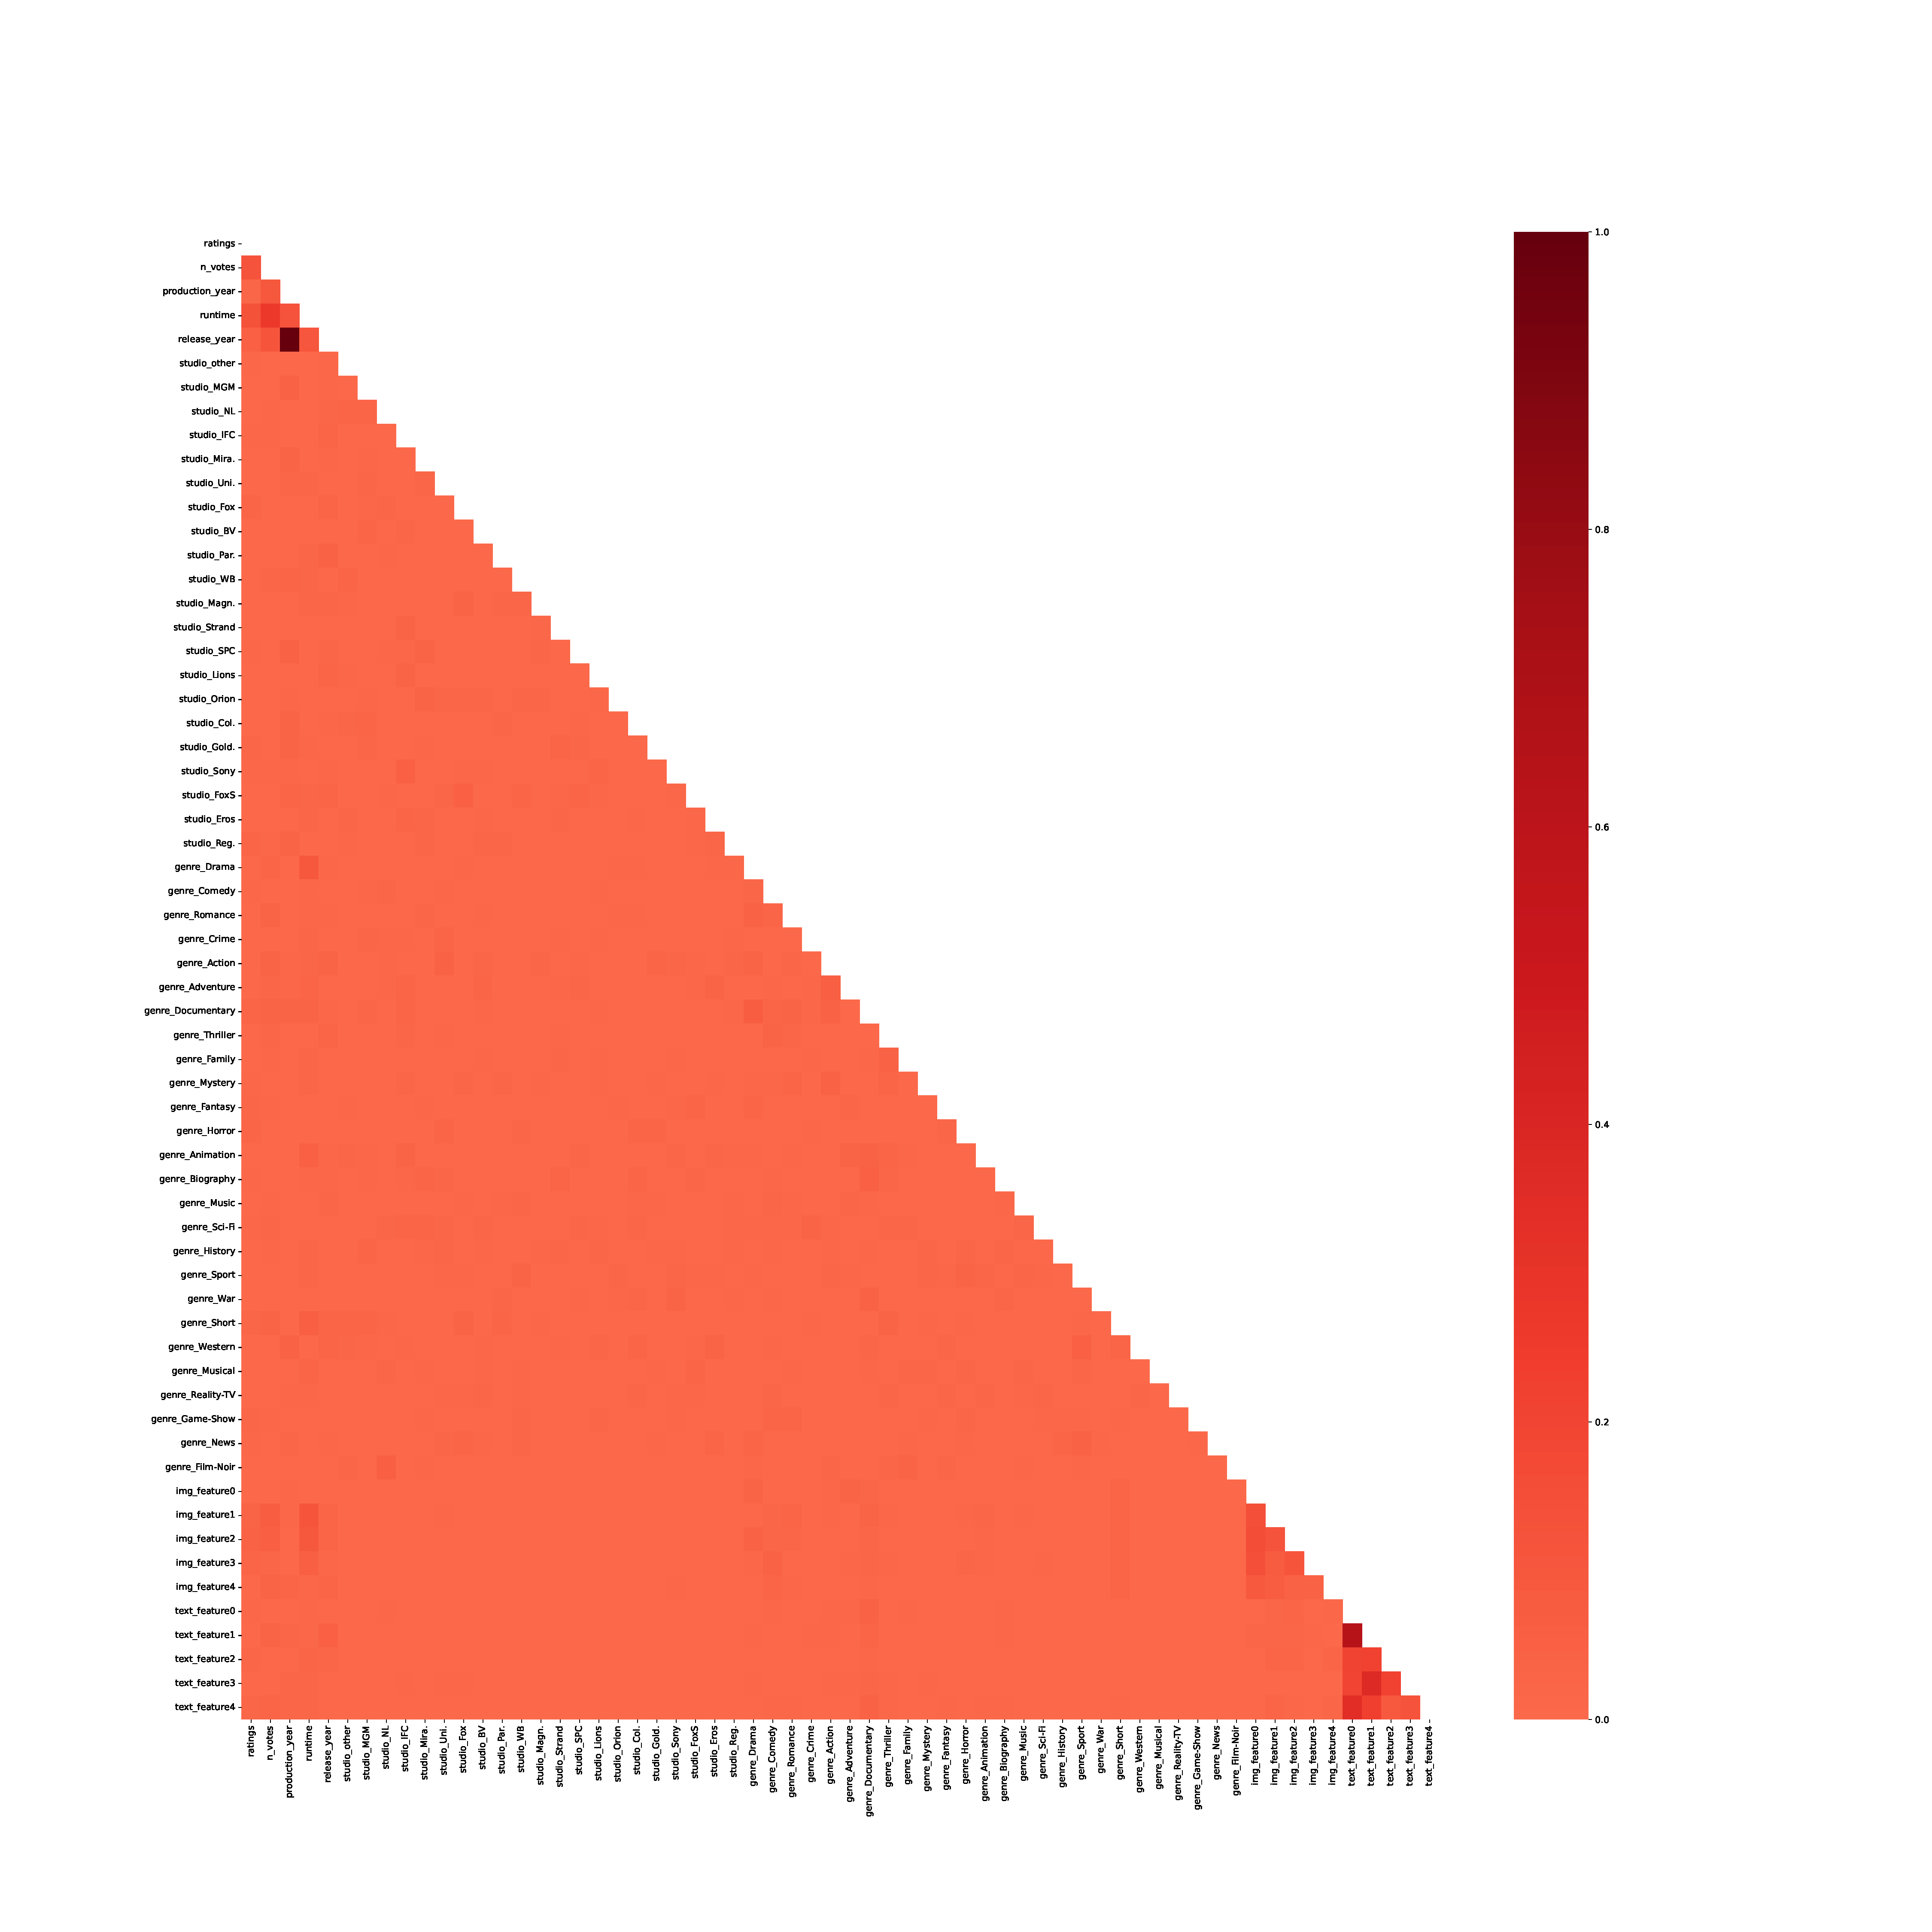
\includegraphics{figures/mi_matrix.tex}
	\caption{Mutual information matrix}
	\label{fig:mi_matrix}
\end{figure}

\begin{figure}[H]
	\centering
	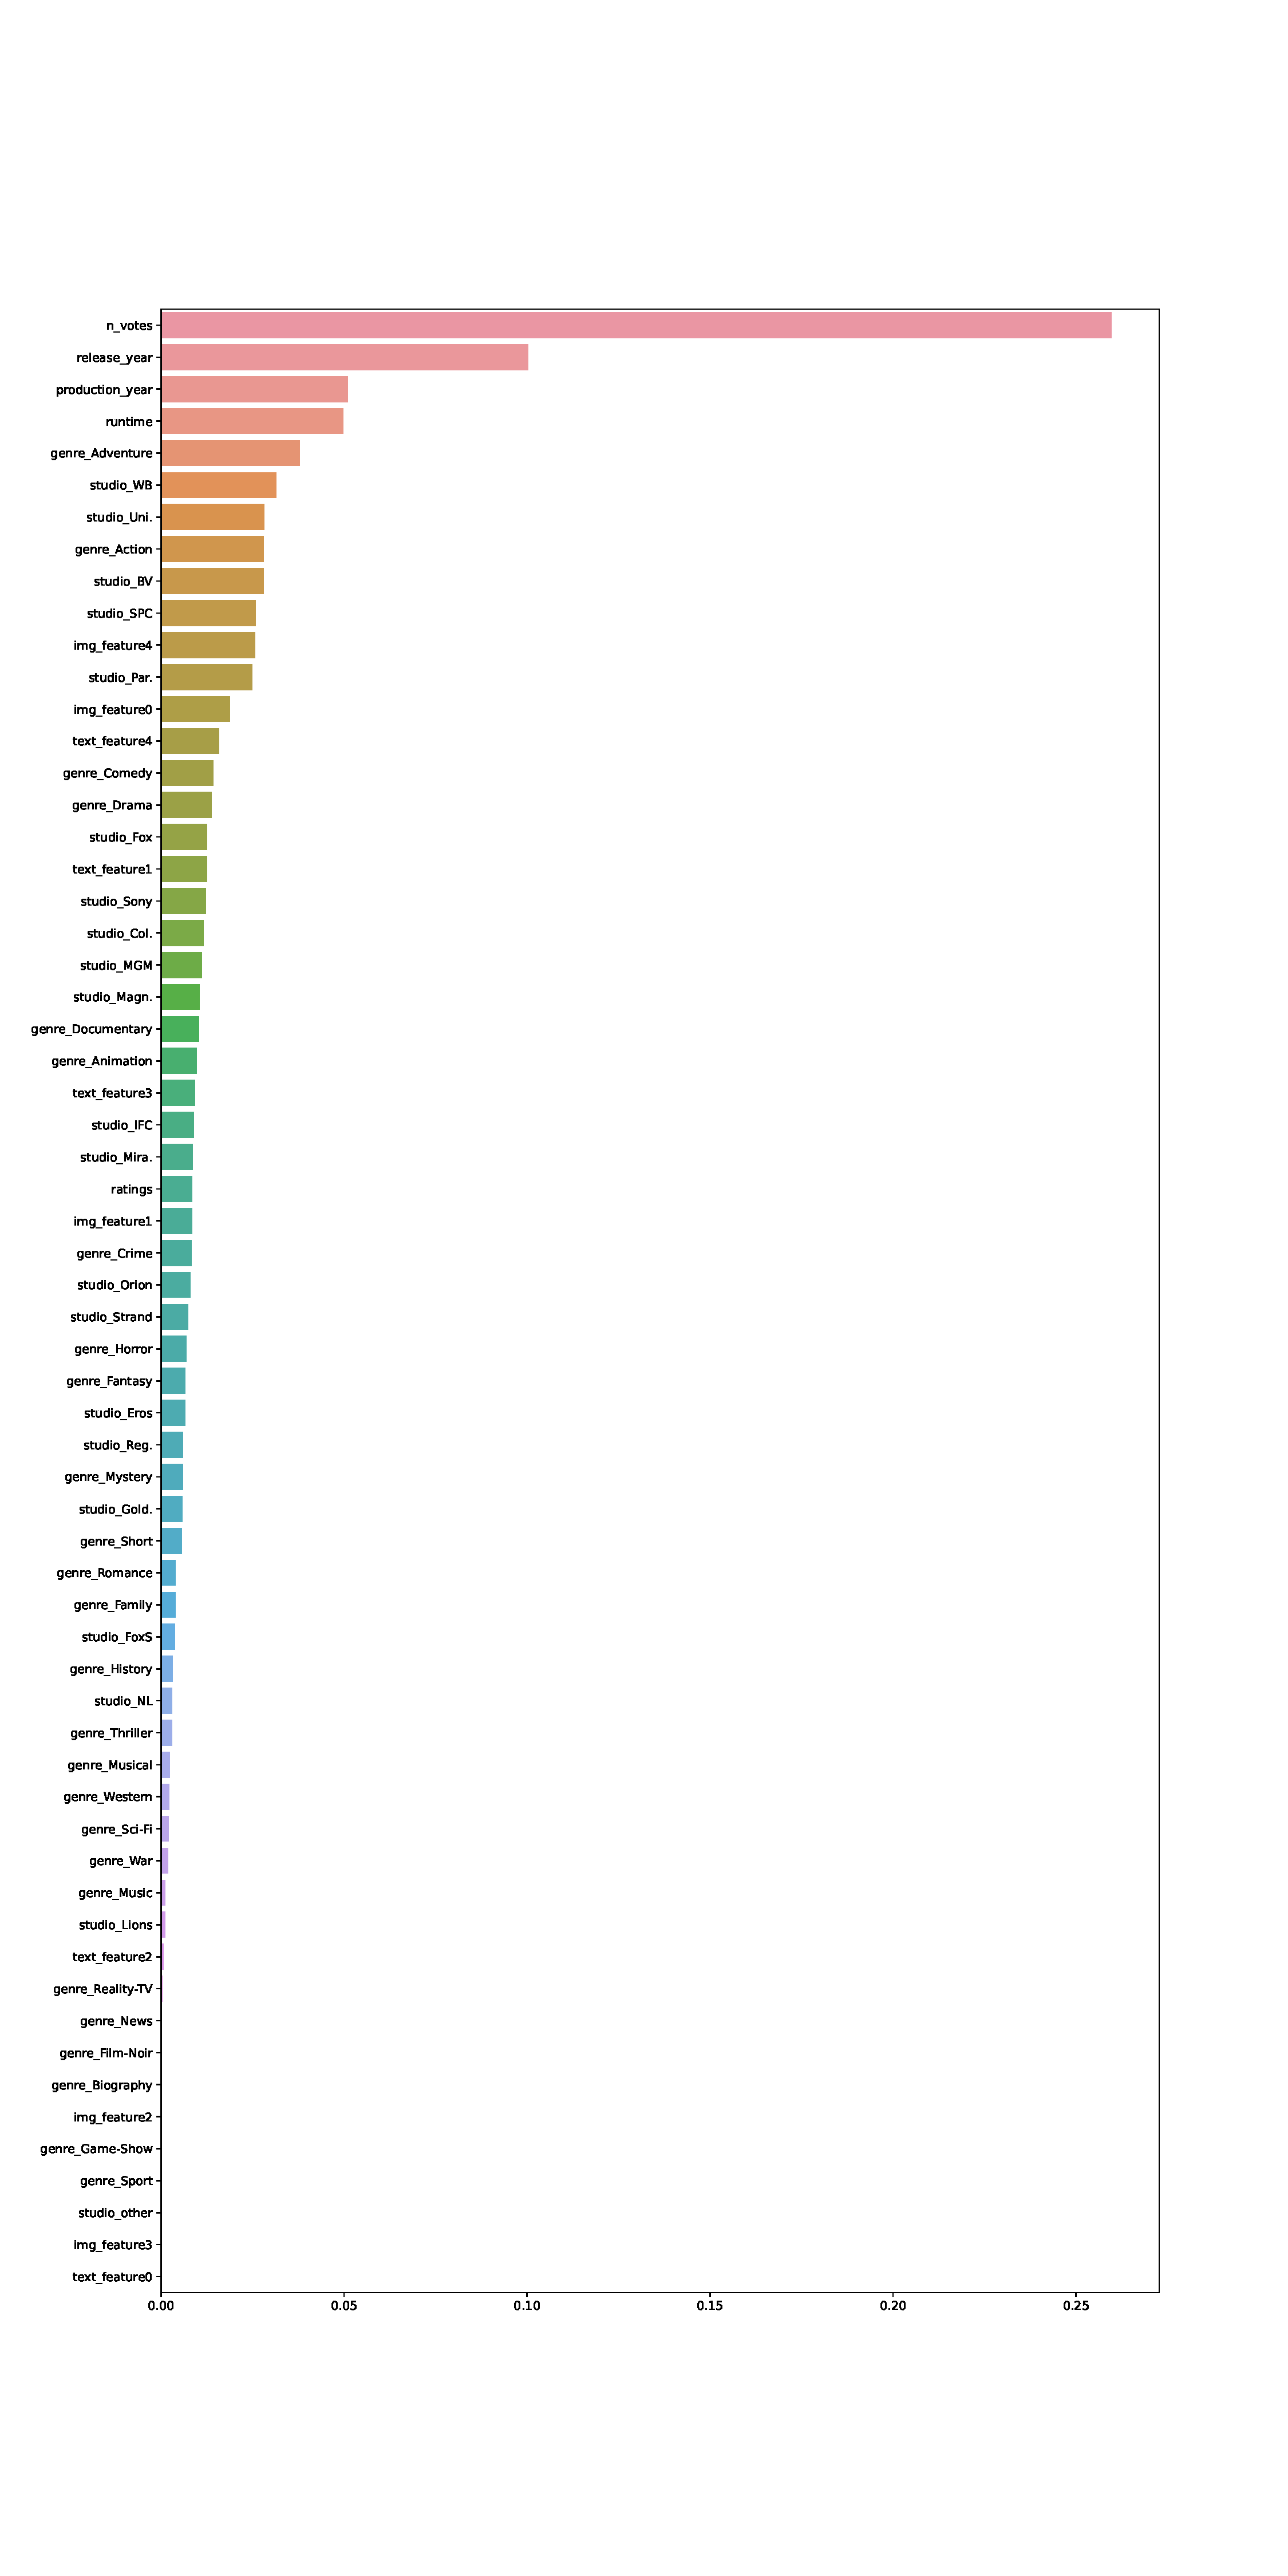
\includegraphics{figures/mi_with_target.tex}
	\caption{Mutual information of each feature with the target variable (revenues)}
	\label{fig:MI_with_target}
\end{figure}

Finally, we decided to test a set of different numbers of features to select our model. We tried to keep respectively the $5$, $10$, $15$, $20$ and $30$ best features that shares the most information with the target.